\documentclass{article}
\usepackage[utf8]{inputenc} % Allow using of åäö, etc.
\usepackage{graphicx} % Add pictures.
\usepackage{verbatim} % Add multiline comments.

% comment about something
\author{Mikael Grön, Anssi Moisio, Visa Koski, Lassi Knuuttila}
\title{Q-learning Project Plan - C++ ELEC-A7150}
\date{\today}

\begin{document}

\maketitle

\tableofcontents
\newpage

\section{Features / Scope}
We are aiming to make an advanced program. Therefore our program will fill
the assignments minimal and optional requirements.

\begin{enumerate}
\item Minimal requirements
    \begin{itemize}
    \item Basic Q-Learning implementation
    \item Simple graphics to visualise learning process
    \item A system where bots will eventually learn how to perform simple
    tasks (such as moving forward) by themselves
    \end{itemize}
\item Optional requirements:
    \begin{itemize}
    \item Application can save learning data to some external file so user
    doesn't lose progress between sessions (suggested)
    \item Ability to fast forward learning steps
    \item Bots can share their knowledge with other bots to speed up learning
    process
    \end{itemize}
\end{enumerate}

To accomplish the optional requirements our program needs to be able to run
at different speeds, so "fast forward learning steps" is possible. This
means that the simulation of the agent can have different speeds.

To have multiple agents that share knowledge, we need a framework where
concurrent computation is possible. \textbf{Does this mean threads or
processes?}

The Q-learning algorithm never finishes, so it needs to be able to be terminated
by the user, therefore threading is needed, for a responsive experience.



\section{Tools}
\begin{tabular}{ll}
Plan                    & Latex \\
Class Structure         & UML \\
Documentation           & Doxygen \\
Compiler                & g++ \\
Compilation manager     & cmake and make \\
Version control         & git \\
Graphics and physics    & Box2D \\
Testing                 & Google Test \\
\end{tabular}



\section{Design and Practice}
\begin{itemize}
\item Regular physical weekly meetings, and possibly some web calls,
in which every developer lists his progress since the last meeting,
and states what the next development goals and its blockers are.
\item Commit only working code. Meaning that all the tests pass.
\item Write code and its tests in tandem, or write test before the actual code.
\item Comment properly your code. Especially important because of Doxygen.
\item Everything written is in English: comments, names, etc.
\item If someone is fast finishing his part, then he can help elsewhere.
\item We try to first make a working version, which then can be further
developed.
\item Limit line length to 80 characters.
\item Tabs are 4 spaces.
\end{itemize}



\section{Preliminary Schedule}
We will have our internal deadlines about 1 to 1/2 weeks before the
courses deadlines, so we have time to iron out possible problems that
were not seen beforehand.

When bigger obstacles arises, the deadlines are adjusted case by case.



\section{Q-learning}
The core Q-learning algorithm is quite simple, so its implementation should
be quite straightforward. The complexity of the problem can raise problems,
so developing the algorithm will also mean the defining of
the problem the Q-learning will solve.

Running the algorithm means having it test different solutions, and finally
maximising the reward, when the agent has learned. The learning means
that the agent runs multiple times over all the possible states,
with all possible actions.

The actor is the thing that is in states from which the actor can do some
actions that move the actor into a new state. After every action the
system gives the actor a reward (a punishment is a negative reward).
The optimal behaviour is determined by how the system gives the actor the
biggest reward.


\subsection{Q-values}
Every combination of states and actions has a Q-value. These Q-values are
initialized all as 0. The optimal action in a state is the action with the
highest Q-value. When the system is learning, an action is performed, and the
Q-learning function updates the Q-value which is associated with the current
state and performed action:

\[Q(s_t, a_t) = Q(s_t, a_t) + \alpha [ r_t + \gamma \cdot max_aQ(s_{t+1}, a)
- Q(s_t, a_t) ]\]

Here $s_t$ is the current state, $a_t$ the current action,
$\alpha$ is the learning rate, $r_t$ is the reward from doing the action,
$\gamma$ is the discount factor, $max_aQ(s_{t+1}, a)$ is the next states
highest possible Q-value.

The Q-learning function makes the Q-values more accurate by testing out
the combinations of states and actions in the system. The Q-learning is an
optimisation method that will find an optimal path which gives the maximum
reward. The best path is the global maximum, but there can exist local maxima.
The local maxima can be avoided by introducing random actions in the learning
process. If the Q-learning has found a local maximum a random action will
hopefully try out something that moves to the global maximum.

Theoretically the exact Q-values are found by running the learning process
for an infinitially long time. This is not practical (duh), so approximate
Q-values are enough. The learning needs to be terminated from outside, when an
satisfactory accuracy is achieved.

To get accurate Q-values, the different combinations of states and actions
need to be tested multiple times during the learning process.
The number of Q-values are the number of states times the number of actions
in every state. Having a smaller amount of Q-values leads to a shorter learning
time. More Q-values can lead to more complex behaviour for the learned actor.
This depends on the system.


\subsection{Modelling of Agents}
We model agents as a combination of sensors and actors. The sensors determine
which state the agent is in, and the actors can perform actions.
We limit our systems to be two dimensional (2D), meaning the world and agents
are 2D. We will implement our program to support other 2D systems, but we
will start by studying a simple case of the agent in the picture:

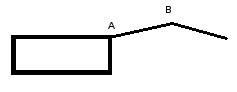
\includegraphics[width=0.8\textwidth]{simple_agent}

We will model this agent that moves trough a flat 2D world.
The agent gets a positive reward when it moves to the right, and a negative
reward when it moves to the left.

The agent has a body and an arm. The arm consists of two beams and two joints
(A and B). The joints angles determine the state of the actor, and actions are
performed by rotating the beams, changing the joints angles.
Both joints can move 360$^\circ$ continuously, but we need to quantisize
the angles, so we can have a limited amount of states. We can also be wise
gods and limit the angle the joints can move. We can see that in our agent's
case that the arm will not affect the state if it flails in the air, not
touching the ground. Also we say that the beam between the joints can not
occupy the same space as the body. Therefore we can limit the joints
permitted angles.

We limit the A joint to move 135$^\circ$, and the B joint to move
270$^\circ$. We quantisize the A joints angle into $2^4$ steps, and
the B joints angle into $2^5$ steps. This gives the actor
$2^4 \cdot 2^5 =$ \textbf{512 states}. The smallest angle registered at
the joint, due to the quantization, is
$135^\circ / 2^4 = 270^\circ / 2^5 \approx 8.4^\circ$.
The angle can be more precise, when simulating the agent, but the
Q-learning algorithm will just "see" the quantizised angle.

A joint can be moved, by performing an action. We limit the movement to be
just one speed, which is one quantization step. A joint can only move
clockwise, counter-clockwise or not move at all. Multiple joints rises the
possible actions to be 3 to the power of the number of joints. Our
agent has two joints, therefore there is $3^2$ = \textbf{9 actions} to
perform in a state.

The number of Q-values is states times actions. Therefore there is
$512 \cdot 9$ = \textbf{4608 Q-values}. This should be a manageable
amount to use the Q-learning algorithm on. If a Q-value is a float,
which is 4 bytes, then the Q-values will occupy 18KB of memory.
Thus the memory size would be tolerable, even when having multiple agents
at the same time learning.

The analysis of the number of Q-values could be too high or low, but that
can be adjusted when trying to run the algorithm.



\section{Class Structure}
The main divide of the program is; learning and simulation. The
simulation and the learning parts communicate with each other mainly by the
learning part telling the simulation to do an action. The simulation will then
simulate the action, returning the new simulated change of the agent, to the
learning part. The learning part evaluates the simulated change, determining
what the reward for the performed action was, updating the Q-value.

In other words, the simulation part contains the world and the body of the agent.
The learning part contains the "brain" of the agent.

Most of the programs classes are dynamically created, aka. template classes.

\textbf{INSERT UML PICTURE}

\textbf{The subsections under will describe the UML picture.}


\subsection{Agent Simulation Initialization}
Loads agent parameters from file and sets the learning and simulation parts.


\subsection{Q-learning}
The Q-learner class can inherit the Agent class or otherwise get the information
what kinds of states and actions are applicable and what the sensors can detect
and initialize itself accordingly. It will initialize its Q-table from a file or
as some pre-determined values, e.g. zeros.

The basic functionalities are: choosing an action based on the current state and
the Q-table, getting a reward based on action, and updating the Q-table based on
the reward. These functionalities will each consist of multiple functions.

To choose an action will be a major part of the Q-learning implementation. An
example of the involved functions could be:
\begin{itemize}
  \item getQValue(state, action) function that returns the Q-value of a state-
    action pair.
  \item maxValue(state) returns the maximum Q-value of the actions of this state
  \item bestAction(state) compares actions (calls maxValue which in turn calls
    getQValue) and returns the best for a given state
  \item getRandomAction() returns a random action
  \item getAction(state) will decide which action is chosen. It will call
    bestAction(state) and/or getRandomAction() depending on epsilon.
\end{itemize}
Choosing the action may be partly random. The value of epsilon will determine to
what degree the action is random; if epsilon is zero, the chosen action is always
the action with a maximum Q-value. Simple way to use epsilon would be to set it
to be some positive constant, e.g. 0.1. A more advanced use of epsilon is to have
it approach zero as the learning process converges.

Learning consists in the abstract of getting rewards and updating the Q-table
according to rewards. Its basic functions should include:
\begin{itemize}
  \item getReward(parameters from the simulation) will evaluate an action based
  on what happened in the simulation when the action was performed. The evaluation
  will be based on predetermined values; what the agent should do in the world,
  what are her highest goals and what is the meaning of her existence, e.g. move
  right.
  \item updateQValue(state, action, qvalue) will call getReward and update the
  Q-value of the given action accordingly
\end{itemize}

There should also be functions to manage the Q-table data, so that the Q-table is
saved when the program is closed: saveQTable, loadQTable, and to show the Q-table:
printQTable.

The agents have different parameters, therefore all data structures and classes
need to support dynamic creation. The Q-table that contains all state-action pairs
and the Q-values could be for example a vector of state-action pair objects. These
objects contain the Q-value as an attribute.


\subsection{Simulation}
\textbf{MORE CONTENT}
The simulation is divided into the graphics and the physics...bla bla blaa...



\section{Distribution of Roles}
Mikael and Anssi will implement the learning part.
Visa and Lassi will implement the simulation part.

\textbf{MORE CONTENT: When the UML is created, the roles can better be defined.
  The more exact roles may be feasible to define later thou...}
The Q-learning implementation could be divided (between Mikael and Anssi) for
example to (A)functions that communicate with the simulation (getReward), update
the Q-table (updateQValue, updateQTable) and manage the Q-table data (saveQTable,
loadQTable, printQTable etc.) and (B) functions that choose the action based on
the Q-table.

\textbf{MORE CONTENT: division of the simulation part}


\end{document}
